% 请在下方的大括号相应位置填写正确的节标题和标签,以及作者姓名
\section{能量计算}\label{sec:能量计算}
\sectionAuthor{Jiaqi Z.}

% 请在下方的item内填写本节知识点
\begin{Abstract}
    \item 如何计算体系的能量
    \item K点与截断能测试

\end{Abstract}

在本节,我们将讨论在计算中最重要的一个物理量——\emph{能量}。如果你是要计算吸附或类似的(两个体系相互作用的能量),肯定需要计算两个体系的能量(甚至可能还需要计算更多)。此外,在实际计算的时候,为节省机时,选择合适的精度也很重要(尤其是对那些花钱买机时的课题组而言更是如此)。而考虑精度是否合适的一个标准,就是计算能量的精度。

% 请在正文相应位置填写正确的小节标题(或小小节标题),同时将标签的“节标题”和“小节标题”改为实际内容

\subsection{自洽计算能量}\label{subsec:能量计算-自洽计算能量}

让我们直接看一个例子——计算单晶Si的能量。首先,我们需要构建Si的结构,也就是\code{POSCAR}文件。在\ref{sec:对晶格常数进行优化ISIF=3}一节中我们已经构建了它的结构,这里直接写出其\code{POSCAR}文件:

\begin{lstlisting}[caption=POSCAR]
Si2
1.0
        3.8669745922         0.0000000000         0.0000000000
        1.9334872961         3.3488982326         0.0000000000
        1.9334872961         1.1162994109         3.1573715331
    Si
    2
Direct
        0.750000000         0.750000000         0.750000000
        0.500000000         0.500000000         0.500000000
\end{lstlisting}

首先需要进行\emph{结构优化},具体方法详见\ref{sec:对晶格常数进行优化ISIF=3},这里不再赘述。假设你已经优化完成了,得到了\code{CONTCAR}文件,将其复制到一个新目录下\footnote{建议这样做,当然,如果你原意直接在当前目录下继续计算,覆盖原有的\code{POSCAR}也没错。},将其命名为\code{POSCAR}。我们后续的大多数计算都是围绕这个结构来的。

在此基础上,自洽计算所使用的\code{INCAR}如下:

\begin{lstlisting}[caption=INCAR]
ISTART =  1
ISPIN  =  1
LREAL  = .FALSE.
ENCUT  =  600
LWAVE  = .FALSE.
LCHARG = .FALSE.
ADDGRID= .TRUE.
LASPH  = .TRUE.
PREC   = Accurate
ISMEAR =  0
SIGMA  =  0.05
NELM   =  60
EDIFF  =  1E-5
\end{lstlisting}

其中,有一些参数需要解释一下:

\begin{itemize}
    \item \keywordin{INCAR}{ISPIN}:表示\emph{自旋极化}开关,当设置为\code{1}时表示不开启自旋极化,当设置为\code{2}时表示开启。这一选项是进行磁性材料计算的重要参数,我们将在\ref{sec:磁矩计算}一节详细介绍;
    \item \keywordin{INCAR}{NELM}:表示最大自洽迭代次数,当达到最大次数时,vasp将停止计算;
    \item \keywordin{INCAR}{EDIFF}:表示自洽迭代的精度,单位为eV,当两次自洽前后能量差小于其数值时,表示达到收敛精度,结束计算。默认值为\code{1E-4}
\end{itemize}

其他参数与结构优化保持一致,完成后查看\code{OUTCAR}文件中在靠近最后的位置有类似下面的输出内容:

\begin{lstlisting}[caption=OUTCAR]
FREE ENERGIE OF THE ION-ELECTRON SYSTEM (eV)
---------------------------------------------------
free  energy   TOTEN  =       -10.78671596 eV

energy  without entropy=      -10.78671596  energy(sigma->0) =      -10.78671596
\end{lstlisting}

可以看到,这里面有三个能量。通常来说,由于我们的计算能量更多是讨论它们的相对值而不是绝对值,因此在实际计算时选择某一个特定的能量,并采用同一标准进行计算即可。通常来说,\emph{我们使用第三个能量\code{energy(sigma->0)}作为体系能量}。

\begin{extend}
    既然已经讨论到这里了,我们就简单介绍一下三个能量表示的含义。其中,\code{free energy TOTEN}表示自由能(吉布斯自由能),其表达式为$F=E-TS$,由于我们的计算不考虑温度(绝对零度),因此按理来说,无论熵怎么变化,对能量的影响都没有影响。而事实上,由于我们的计算采用Gaussian展宽(\code{ISMEAR=0}),在实际计算时会引入在费米能级附近变化的电子态,从而引入了误差(具体来说,是引入了“温度”)

    \code{energy without entropy}表示\emph{不考虑熵时的自由能},\code{energy(sigma->0)}表示当展宽趋向于0时的能量。在本例中,这三个能量值相等,但这不总是绝对的。之所以如此,是因为我们计算的Si是半导体,且设置的展宽合理,从而导致电子占据与实际情况接近(在\code{OUTCAR}中,我们可以看到电子的占据情况(\code{occupation})。如果展宽过大(例如在本例中,如果设置\code{SIGMA=1},再次计算能量,则有可能有下面的情况:

    \begin{lstlisting}[caption=OUTCAR]
FREE ENERGIE OF THE ION-ELECTRON SYSTEM (eV)
---------------------------------------------------
free  energy   TOTEN  =       -10.83981213 eV

energy  without entropy=      -10.66813608  energy(sigma->0) =      -10.75397411        
    \end{lstlisting}

    可以发现,三个能量是不相等的。但一般来说,第三个能量(展宽为0时的能量)总是等于前两个能量的平均值。

    此外,当我们使用\code{ISMEAR=-5}(表示正四面体方法时),其计算严格按照费米能级定义,此时的三个能量应该相等。也正因如此,在计算半导体或绝缘体时,由于存在费米能级(电子填充的最高态),因此使用\code{ISMEAR=-5}会得到更准确的结果。但这是以计算效率为代价。也正因如此,\emph{在计算导体时,千万不要使用\code{ISMEAR=-5}计算}!
\end{extend}

\begin{attention}
    在能量计算的时候,通常绝对值是没有意义的,因为这个数值涉及到零点的选择。类似于普通物理(电磁学)中对带电粒子能量的讨论,通常我们选择无穷远处为零势能面,其能量为0,从而得到带电粒子的能量。在这里情况是类似的——能量的零点是可以自由设置的,因此我们没有办法讨论具体的能量值。但\emph{能量的相对值是确定的}。例如,我们永远无法说一个物体的势能是多少(这涉及到零势能面选取),但当讨论势能变化时,无论怎么选取零势能面,其结果都是确定的。

    正因如此,在论文中,我们需要尽量避免出现绝对能量,而使用相对能量(如吸附能、结合能等都是通过\emph{体系能量差值}定义的)
\end{attention}

\subsection{使用能量进行收敛性测试}\label{subsec:能量计算-使用能量进行收敛性测试}

在计算一个体系之前,首先是需要对体系进行收敛性测试,以选择合适的参数,从而兼顾效率和精度。通常涉及到的收敛性测试包括截断能和K点,越高的截断能,越精细的K点,计算得到的精度越高,但这会带来更多的计算机时成本。因此,在进行计算前应该想办法找到合适的精度,这一方法就是\emph{收敛性测试}。

具体来说,所谓收敛性测试,就是通过改变参数做自洽计算,得到体系能量随参数的变化。通常来说,\emph{每原子能量变化在1 meV以下时,表示体系精度收敛},可以进行后续计算。

\subsubsection{截断能测试}

同样还是前面的Si单晶,在实际计算时,我们都是先进行收敛性测试。因此,我们使用最开始的\code{POSCAR}。创建若干个截断能测试目录,并将计算任务复制到里面,改变截断能参数(在这里,我们取200、250、300、350、400、450、500、550、600、650、700),分别计算这些任务,并考察能量变化。

\begin{extend}
    在创建测试目录时,你当然可以直接创建,但更简单的方法是使用\code{for}循环。具体的方法在讲解Linux时的\ref{subsec:简单for循环-一些for循环使用例}一节有详细介绍,这里不赘述。如果你看到这里再回头看那一部分就会发现,当时的例子就是为了解决这一问题。
\end{extend}

计算完之后查看能量随截断能的变化,处理数据如图\ref{fig:能量计算-截断能收敛性测试}所示。可以发现,随着截断能的增大,体系能量逐渐减小(蓝线),但在400 eV之后能量减小得更慢,甚至已经达到了前面所说的收敛标准(每原子能量变化在1 meV以下,见红线),因此,在后续计算时,使用400 eV作为截断能就足够了。

\begin{figure}
    \centering
    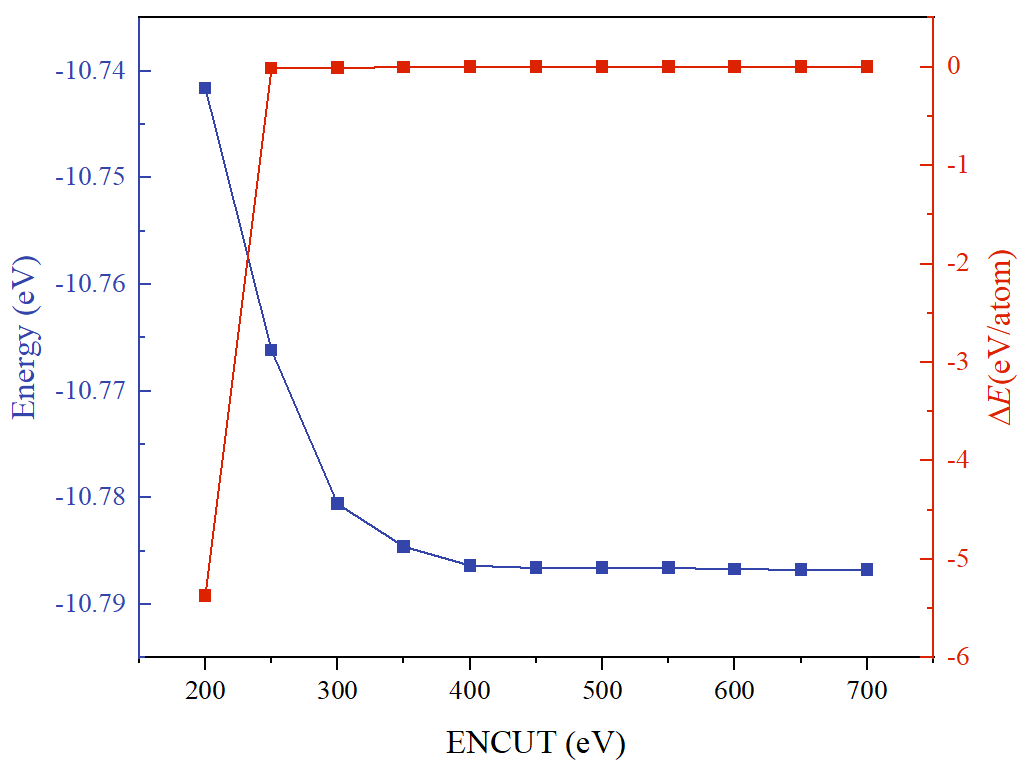
\includegraphics[width=1\linewidth]{VASP计算/静态自洽与电荷密度/能量计算/fig/截断能收敛性测试.png}
    \caption{截断能收敛性测试}
    \label{fig:能量计算-截断能收敛性测试}
\end{figure}

\begin{attention}
    在截断能的选择上,通常有一个理论最小值,也就是你所选择的赝势中\keywordin{POTCAR}{ENMAX}的最大值。设置的截断能必须比这个数值大才有可能保证准确性。例如,在本例中,如果查看我们使用的Si的赝势,里面有\code{ENMAX = 245.345},表明我们计算时所使用的截断能必须比这个数值大。通常情况下,使用\code{ENMAX}的1.3倍到1.5倍是合适的。
\end{attention}

\begin{extend}
    虽然我们多次说明:在计算时应当指定截断能,但事实上\code{ENCUT}本身是有默认值的,这个默认值就是赝势文件中\code{ENMAX}的最大值。尽管如此,对于不同的体系可能会有不同的默认值,在计算时为了统一,还是应当设置\code{ENCUT}。
\end{extend}

\subsubsection{K点测试}

关于K点的测试,方法与截断能完全类似,这里只给出最终结果如图\ref{fig:能量计算-K点收敛性测试}所示。可以发现,当K点取$9\times9\times9$时,体系能量收敛。

\begin{figure}
    \centering
    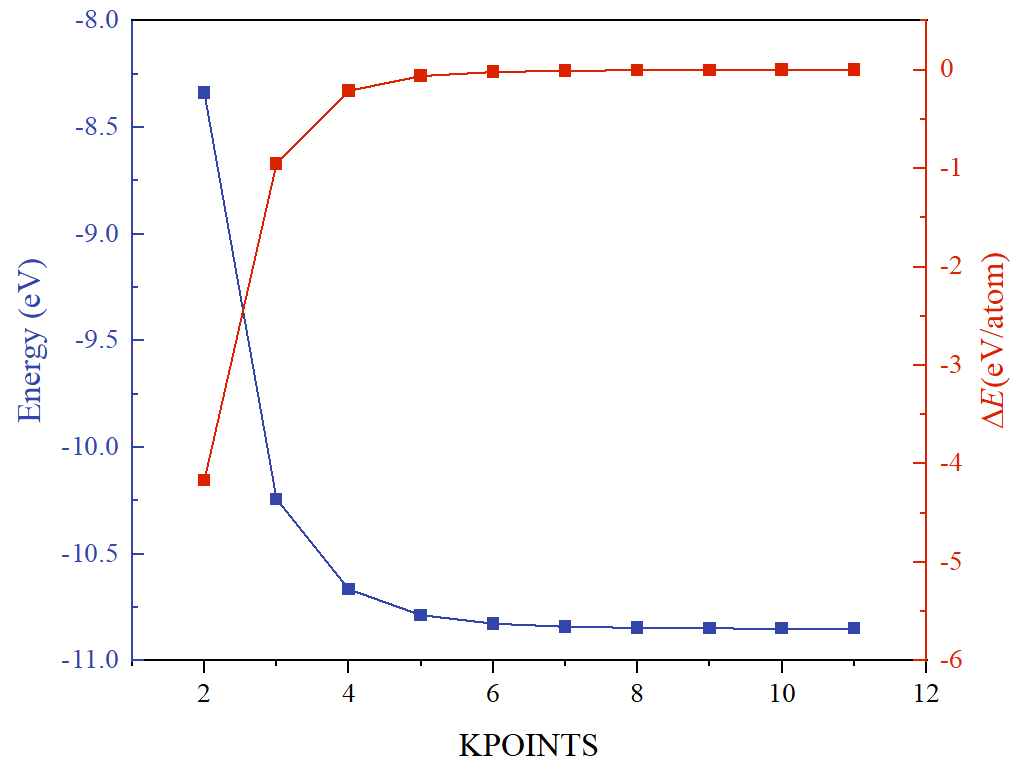
\includegraphics[width=1\linewidth]{VASP计算/静态自洽与电荷密度/能量计算/fig/K点收敛性测试.png}
    \caption{K点收敛性测试}
    \label{fig:能量计算-K点收敛性测试}
\end{figure}

\begin{attention}
    上述收敛性测试的例子仅是一个参考,实际情况还需要结合机时与计算时间综合考虑。此外,在这里我们所给出的结果是计算前用来做参数测试的步骤,在后续教程中,我们都不会进行这一步。其中有一些情况是结合经验选择的参数,有些是做过收敛性测试。在实际计算时,应结合实际情况选择参数。
\end{attention}

% \subsection{错误处理}\label{subsec:节标题-错误处理}
% % 请在本节列出可能遇见的错误与解决方法

% \subsubsection{错误1}

% \subsubsection{错误2}

% \subsubsection{错误3}